\section{Aprendizaje profundo}

\subsection{Redes neuronales}

Una red neuronal se llama así porque los científicos intentaron modelar el cerebro en código informático. El objetivo final es crear una “inteligencia general artificial”, en otras palabras un programa que puede aprender todo lo que una persona podria aprender.

Las redes neuronales artificiales son una clase de algoritmos de aprendizaje máquina que aprenden de los datos y se especializan en el reconocimiento de patrones (\cite{rosebrock2017deep}).

Una red neuronal es una función flexible que adapta de manera autónoma su comportamiento para satisfacer la relación entre la entradas y los resultados esperados y se ha denominado como un aproximador universal (\cite{goyal2018Deep}).

\subsection{Perceptrón}

Rosenblatt publicó el algoritmo seminal Perceptron: este modelo podía aprender automáticamente los pesos necesarios para clasificar una entrada.

Perceptron toma n entradas y produce una única salida binaria si la suma es mayor que el valor de activación. Se dice que la neurona se "dispara" siempre que se excede el valor de activación y se comporta como una función escalonada (\cite{goyal2018Deep}).

Minsky y Papert demostraron que un perceptrón con una función de activación lineal es simplemente un clasificador lineal, incapaz de resolver problemas no lineales (\cite{rosebrock2017deep}). El ejemplo canónico de un problema no lineal es el conjunto de datos XOR Figura \ref{fig:xor}.

Perceptron se puede convertir fácilmente en un algoritmo en línea que procesa un flujo de ejemplos, actualizando el vector de peso solo si el último ejemplo recibido está mal clasificado. Se garantiza que el perceptrón convergerá en una solución si los datos de entrenamiento son linealmente separables, pero de lo contrario no convergerán(\cite{flach2012Machine}).

\begin{figure}[H]
    \centering
    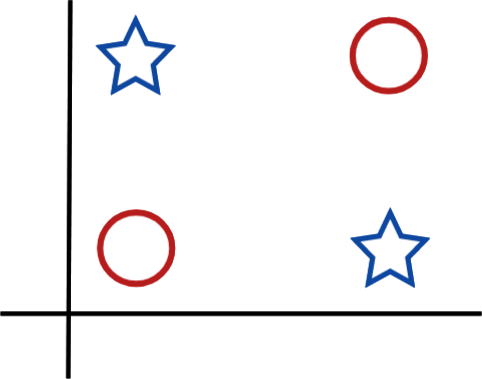
\includegraphics[width=0.8\textwidth]{MarcoTeorico/imgs/XOR.png}
    \caption{Problema XOR, no es linealmente separable.}
    \label{fig:xor}
\end{figure}
